%****************************************************
%	CHAPTER 2 - LIT REVIEW
%****************************************************
\chapter{Literature Review}
\label{ch:lit_review}

%====================================================
\section{Antarctica and the Southern Ocean}
\label{sec:ch2.section1}
%----------------------------------------------------

Historically, Antarctica and the Southern Ocean that surrounds it have been under observed by the global scientific community, and the observations that have taken place are biased towards certain sectors and times of the year (\cite{kennicuttSustainedAntarcticResearch2019}). There are many reasons for this bias, ranging from the extreme isolation and difficulty associated with reaching the region, sampling and observation coinciding with relief voyages that take place during the austral summer in sectors in proximity of the research stations, and the observational bias towards the Northern Hemisphere often seen in scientific research. In recent years this has begun to change, with efforts such as the 2017 \ac{PIPERS} cruise that took place in Autumn (\cite{ackleySeaiceProductionAir2020}) and the \ac{SCALE} Winter 2017 (\cite{vichiCruiseReportTrack2018}), \ac{SCALE} Winter 2019, \ac{SCALE} Spring 2019 (\cite{ryan-keoghSCALEWIN19SCALESPR19Cruise2022}) and \ac{SCALE} Winter 2022 cruises that took place aboard the research vessel \textit{S.A. Agulhas II}, which both addressed under observed seasonal periods (\cite{vichiIndicatorSeaIce2022}).

The Earth's environment is a massively complex and interconnected system and the Antarctic seasonal ice cycle is a critical component of this system. It is known that global albedo, atmospheric and oceanic circulation and ocean productivity are all directly linked to the Antarctic (\cite{eayrsUnderstandingSeasonalCycle2019}), but the full extent of these relationships are still under investigation. Due to the biased and limited observations of the Antarctic, the models used to represent the region are parametrised on these skewed data, leading to inaccuracies and uncertainties in the models. Without a deeper understanding of each part of the global system, it is impossible to accurately model or predict the system's response to disturbances such as anthropogenic climate change or forecast future behaviour.

%====================================================
\section{Antarctic Seasonal Ice Cycle}
\label{sec:ch2.section2}
%----------------------------------------------------

The Antarctic seasonal ice cycle is one of the largest environmental cycles on Earth, with sea ice coverage reaching a minimum of approximately 3 x $10^6$ km$^2$ in the summer months, increasing to its maximum of approximately 18 x $10^6$ km$^2$ in the winter months, an increase in area greater than of the Antarctic continent itself (\cite{parkinsonSouthernOceanSea2004}). The cycle of change in ice extent is asymmetrical, characterised by a rapid melting and retreat in the springtime, followed by a gradual growth and expansion during autumn, at almost half the rate of the spring retreat (\cite{gordonSeasonalitySouthernOcean1981}). This behaviour is contrasted by the Arctic, where the rate of melt and growth is approximately symmetrical around the region throughout the year (\cite{walshAnalysisArcticSea1979}). This behaviour highlights that despite both the Arctic and Antarctic being polar regions, their dynamics and processes are inherently different from each other and cannot be generalised across both regions.

%----------------------------------------------------
\begin{figure}[H]
\centering
\begin{minipage}{.5\textwidth}
    \centering
    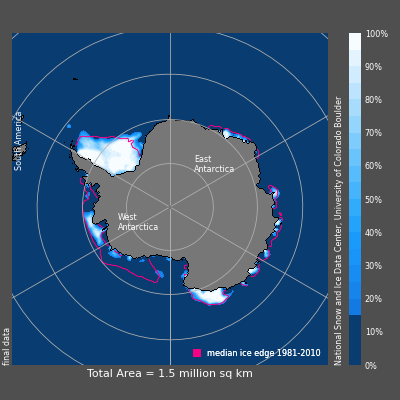
\includegraphics[width=0.95\linewidth]{figs/ch2/sic_feb.png}
  \end{minipage}%
  \begin{minipage}{.5\textwidth}
    \centering
    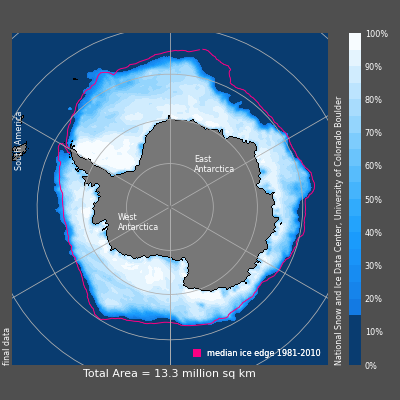
\includegraphics[width=0.95\linewidth]{figs/ch2/sic_sept.png}
  \end{minipage}
  \caption{\textbf{Sea Ice Extent.}}{Average sea ice concentration for February (left) and September (right) 2024, the annual minimum and maximum respectively. Taken from \textcite{BrowseImageSubset}.}
  \label{fig:ice_exten}
\end{figure}
%----------------------------------------------------

The drastic change in sea ice extent throughout the year has a significant impact on the Antarctic climate and environmental conditions. The presence of sea ice increases the albedo of the region, reduces the heat exchange between the ocean and atmosphere, and increases the salinity of the surrounding seawater. Sea ice also directly interacts with wind and wave activity, with the presence of ice dampening wave energy, wave activity influencing ice formation and growth, and wind driving ice drift (\cite{roachPhysicsSeasonalSea2025}). Drivers of the Antarctic seasonal ice cycle have been identified, such as wind, ocean-ice interactions and ocean-atmosphere interactions, but further understanding of these mechanisms is required to fully explain the variability of the cycle (\cite{eayrsUnderstandingSeasonalCycle2019}).

On the edge of the continually growing and shrinking ice cover lies the \ac{MIZ}, one the most dynamic and poorly understood regions of the Antarctic.

%----------------------------------------------------
\subsection{Marginal Ice Zone}
\label{subsec:ch1.section2.subsec1}

The \ac{MIZ} is widely accepted to be the transitional region where the open ocean transitions to consolidated ice cover. This region is characterised by constant interactions between ice above, the ocean surface below and the atmosphere and ocean. There is no universally accepted definition of the \ac{MIZ}, which leads to difficulties in understanding and comparing studies on the area by different authors who have varying definitions of the \ac{MIZ}. \textcite{wadhamsMechanismFormationIce1983} gives a definition of the \ac{MIZ} based on three distinct zones, characterised by the width if the zones and the size and thickness of the ice floes present within them. The definition given by \textcite{squireMarginalIceZone2022} is based on the seasonality, variability and dynamics of the region, and does not provide specific boundaries or physical characteristics of the \ac{MIZ}. \textcite{vichiIndicatorSeaIce2022} states the \ac{MIZ} is generally seen as the region where \ac{SIC} is between 15\% and 80\%, but this simple threshold based definition has proved to be a less reliable for the Antarctic, where ice drift and wave activity has been reported in areas classified as having 100\% ice cover. They propose an alternative indicator of the \ac{MIZ} based on the variability of \ac{SIC} over time, and that the ice types and their associated properties are potentially of greater importance in defining the \ac{MIZ} than \ac{SIC} alone.

Due to its location, the \ac{MIZ} is a highly dynamic region, leading to greater variability in its conditions, processes and dynamics when compared to other ice-covered regions. Various types of ice make up the \ac{MIZ}, but the correlation between \ac{SIC} and ice type (frazil, pancake, grease, etc.) have not been fully characterised, especially in their formation stages (the Autumn and Winter months) (\cite{vichiIndicatorSeaIce2022}).

During the summer months the \ac{MIZ} predominantly consists of large floes, capable of reaching sizes in the hundreds of meters, formed by the seasonal pack ice breakup. This is contrasted by the winter months, when the \ac{MIZ} is dominated by a huge number of smaller pancake ice floes and various other types, such as brash, grease and nilas ice (\cite{alberelloPhysicalModelWave2021}).

%----------------------------------------------------
\begin{figure}[H]
    \centering
    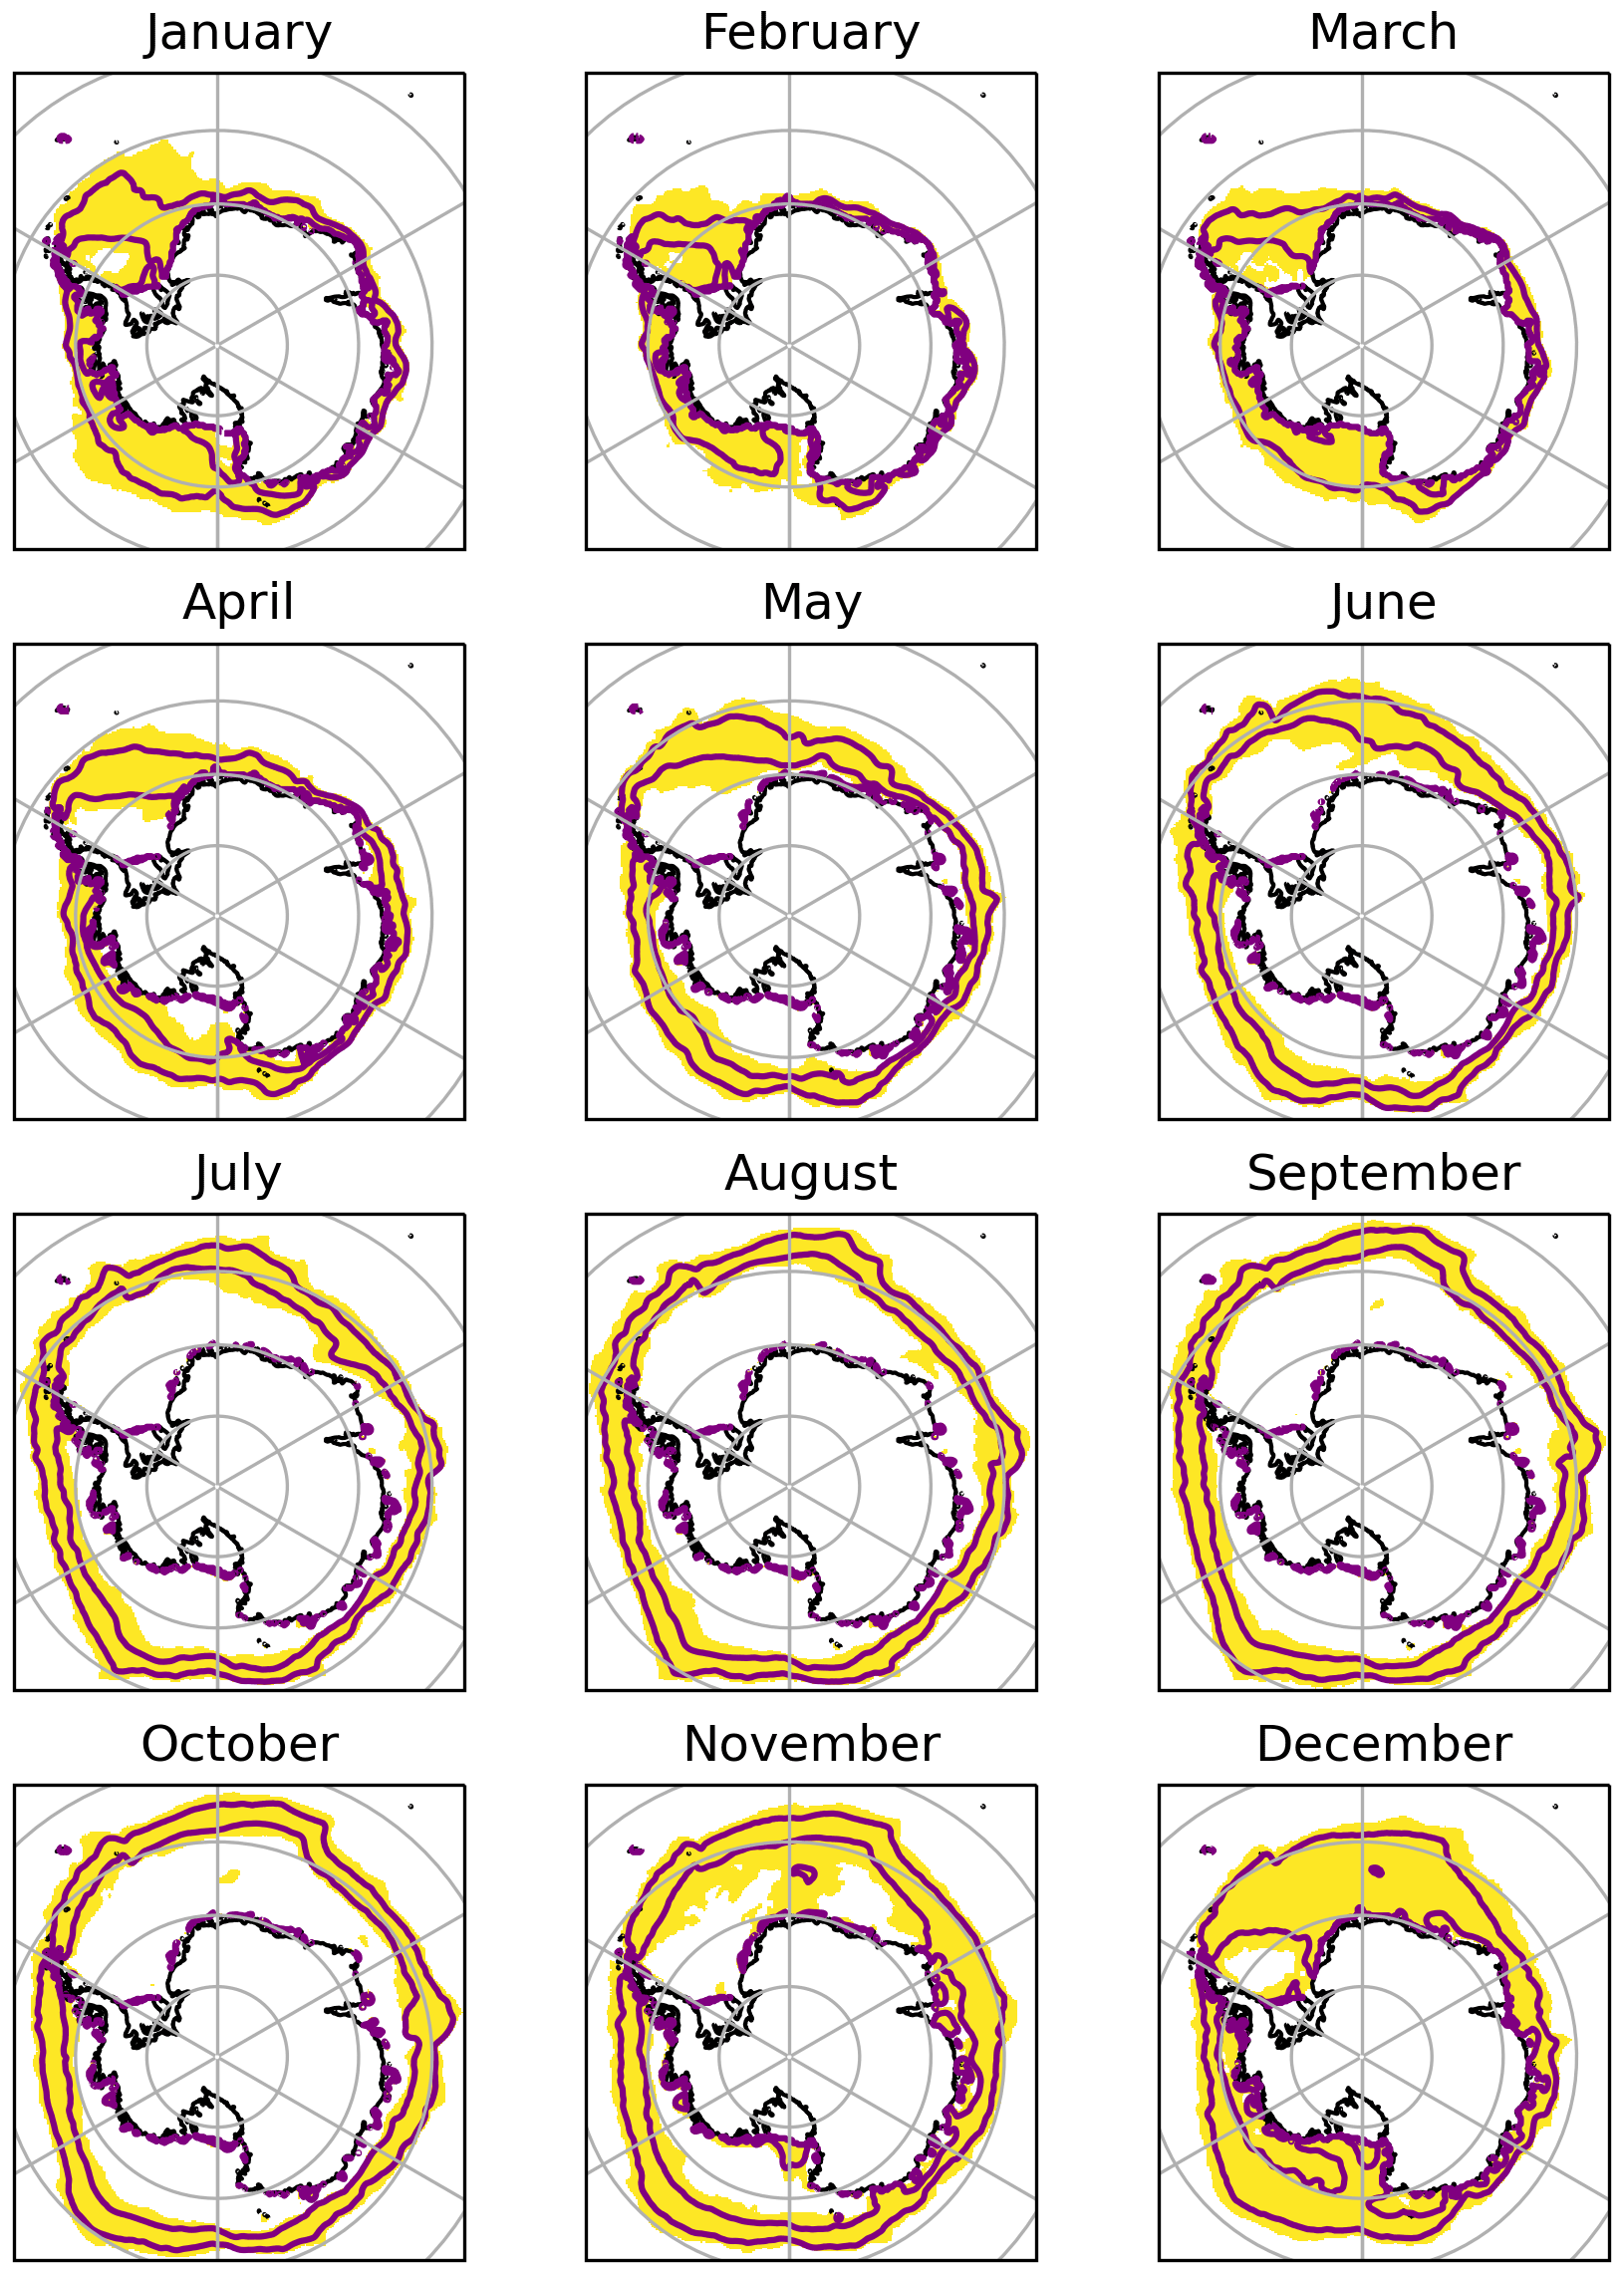
\includegraphics[width=0.6\textwidth]{figs/ch2/miz.png}
    \caption{\textbf{2016 Monthly MIZ.}}{Yellow region represents MIZ as determined by the alternative indicator proposed by \textcite{vichiIndicatorSeaIce2022}, the purple lines represent MIZ extent as determined by the traditional SIC threshold. Taken from \textcite{vichiIndicatorSeaIce2022}.}
    \label{fig:miz}
\end{figure}
%----------------------------------------------------

As seen in Figure \ref{fig:miz}, the \ac{MIZ} undergoes huge seasonal variability in both extent and location. In September, when sea ice extent reaches its maximum, the \ac{MIZ} exists as a narrow band at the edge of the ice extent. As the ice begins to retreat during the spring months, the \ac{MIZ} expands rapidly, and in December, what once was consolidated ice cover surrounding Antarctica is classified as the \ac{MIZ}.

%----------------------------------------------------
\subsection{Pancake Ice}
\label{subsec:ch2.section2.subsec2}

Pancake ice is the name given to roughly circular, consolidated ice floes, seen below in Figure \ref{fig:pancake_floes}, commonly found in polar marginal ice zones where turbulent wave and wind activity is present during the ice formation (\cite{doblePancakeIceFormation2003}). The growth and fusion of pancake ice is the main driver of pack ice formation in the Antarctic.

%----------------------------------------------------
\begin{figure}[H]
    \centering
    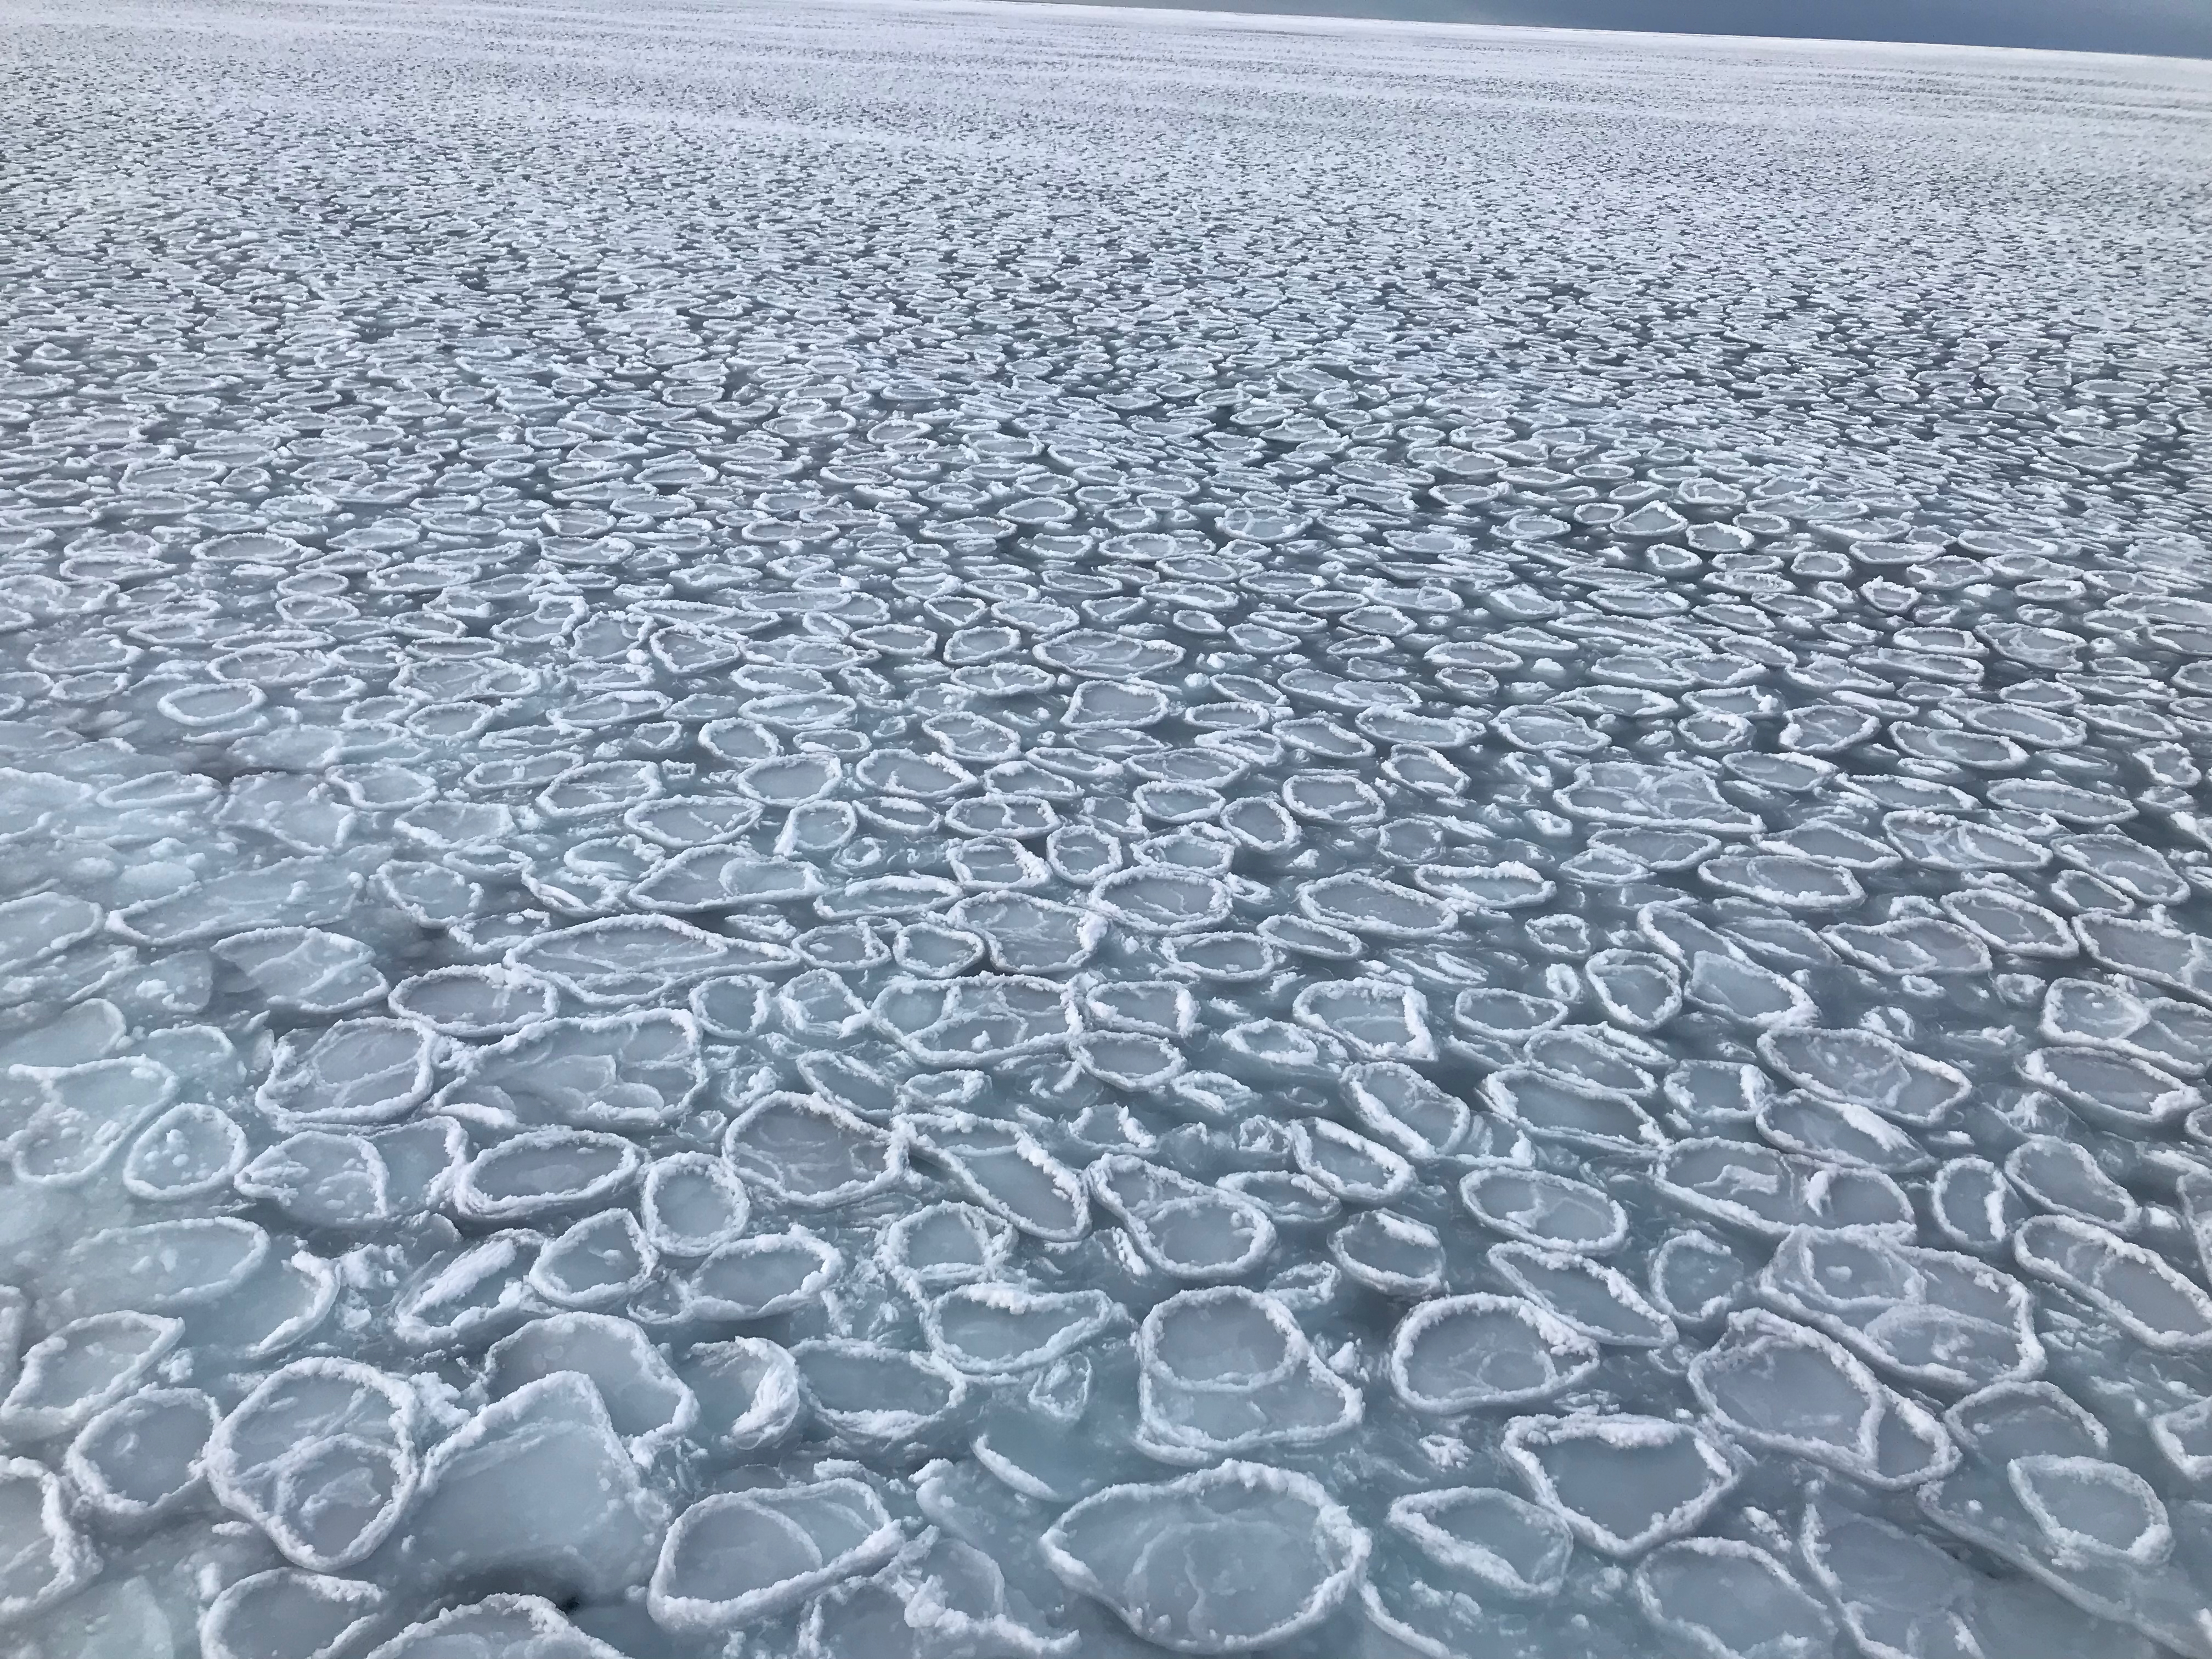
\includegraphics[width=0.5\textwidth]{figs/ch2/pancake_floes.jpg}
    \caption{\textbf{Pancake Ice Floes in the MIZ.}}{Small pancake floes in the early stages of formation. Captured during the SCALE Winter 2019 cruise aboard the \textit{S.A. Agulhas II}. Image credits: R.A. Verrinder.}
    \label{fig:pancake_floes}
\end{figure}
%----------------------------------------------------

%----------------------------------------------------
\subsection{Pancake Ice Formation}
\label{subsec:ch2.section2.subsec3}

Wave activity and, to a lesser degree, wind activity are necessary for the formation of pancake ice, as the continuous motion provided by the wind and waves promotes the formation of frazil and grease ice over nilas ice (\cite{shenConceptualModelPancakeice2001}). This prevents continuous sheets of ice from forming over the ocean.

\cite{shenConceptualModelPancakeice2001} propose a three-stage model of pancake ice formation:

\begin{enumerate}
    \item Grease-ice stage
    \item Pancake formation stage
    \item Composite pancake stage
\end{enumerate}

In the grease-ice stage, the ocean is supercooled, leading to the formation of frazil crystals. Wind and/or wave agitation causes these frazil crystals to collide and adhere to each other, forming miniature disc-like frazils. These newly formed frazils are driven together by the high-frequency components of the wave spectrum to form grease ice, which absorbs the energy of the high-frequency components.

%----------------------------------------------------
\begin{figure}[H]
    \centering
    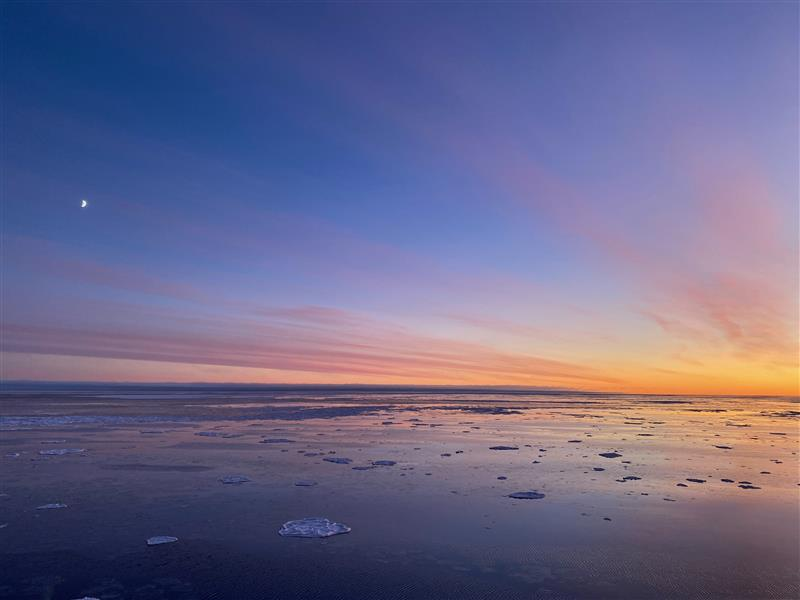
\includegraphics[width=0.5\textwidth]{figs/ch2/grease.jpeg}
    \caption{\textbf{Grease Ice in the MIZ.}}{Grease ice can be seen floating in the bottom right of the frame. Captured during the SCALE Winter 2019 cruise aboard the \textit{S.A. Agulhas II}. Image credits: R.A. Verrinder.}
    \label{fig:grease}
\end{figure}
%----------------------------------------------------

Frazils continue to form and adhere to each other beneath the grease ice layer in the pancake formation stage, leading to an increase in the buoyancy of the accumulated crystals. This increased buoyancy causes the disk-like frazils to rise, exposing them to cold air above the surface of the ocean, resulting in the formation of an ice sheet. Throughout this, the wave motion limits the pancake footprint size and floe-floe collisions result in the formation of ridged edges. The high frequency components of the wave spectrum initially dictate the size of the pancake floes, as the energy from these frequencies is consumed by interactions such as collisions and rafting, lower frequencies begin to drive floe creation and interaction. These lower frequencies result in larger pancake floes being able to form, like the floes seen in Figure \ref{fig:pancake_floes}.

%----------------------------------------------------
\begin{figure}[H]
    \centering
    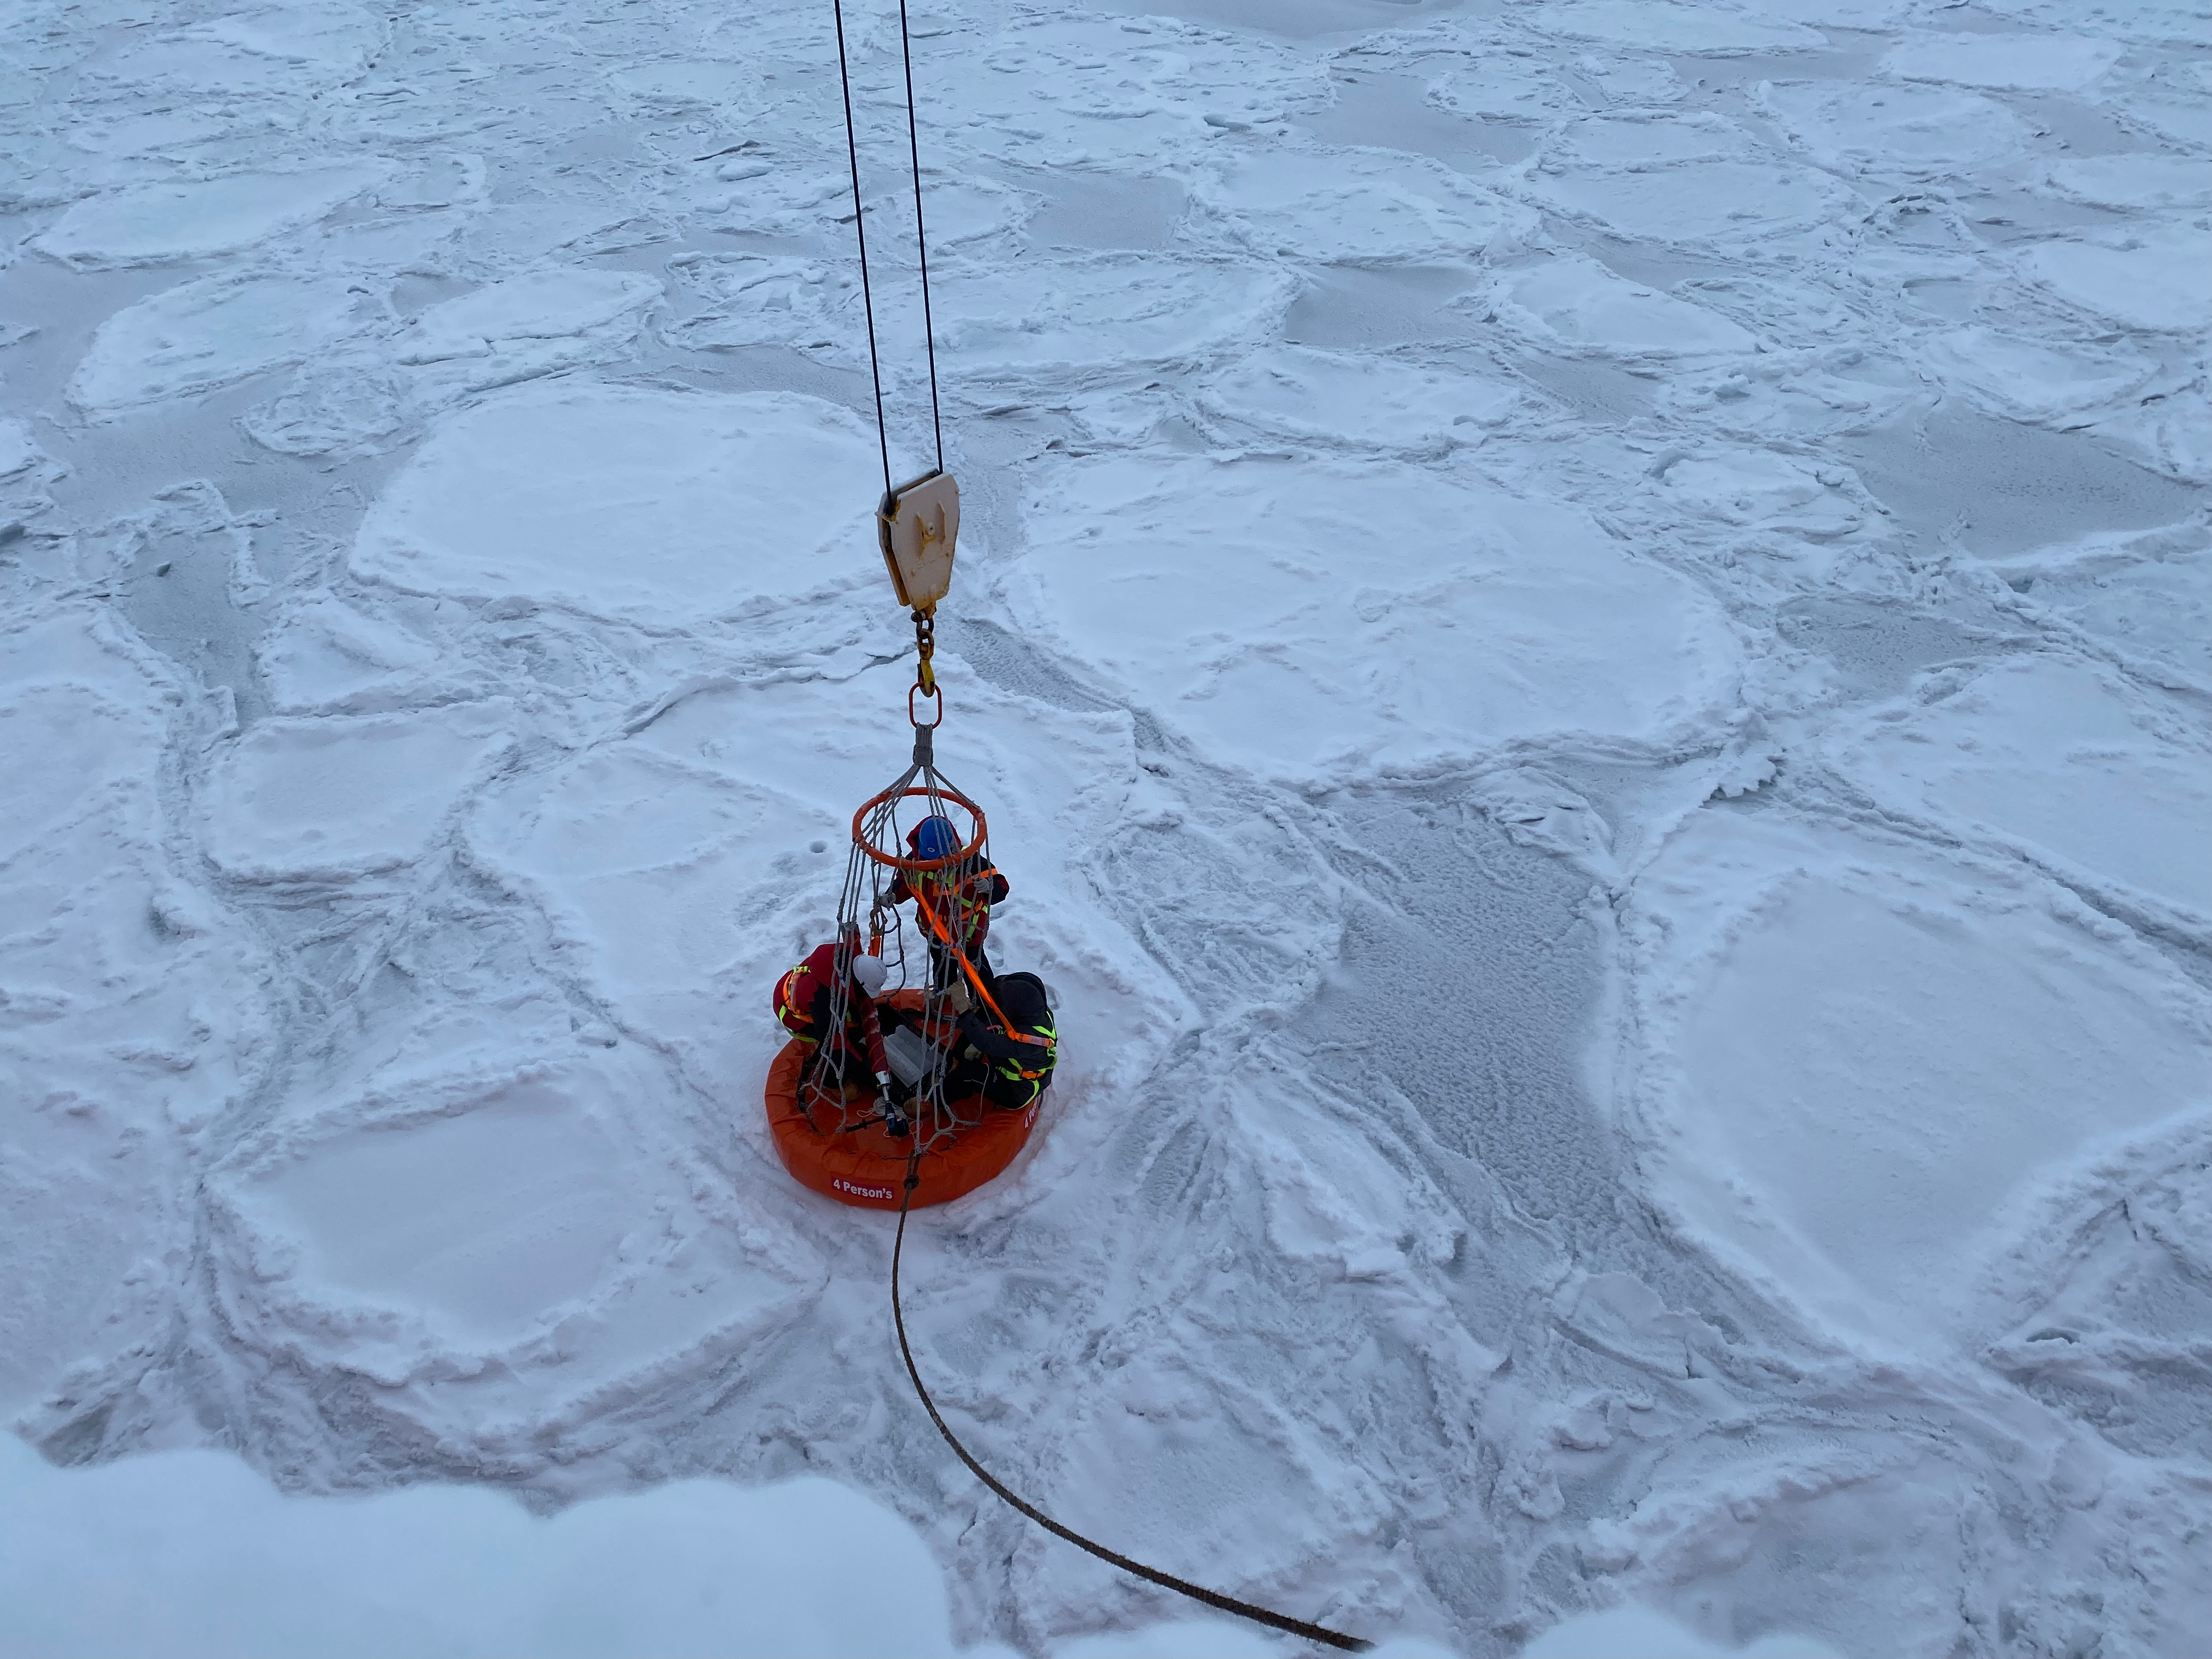
\includegraphics[width=0.5\textwidth]{figs/ch2/pancake_sheet.jpeg}
    \caption{\textbf{Pancake Floe Sheet.}}{Pancake floes fused together to create a consolidated ice sheet. Captured during the SCALE Winter 2019 cruise aboard the \textit{S.A. Agulhas II}. Image credits: R.A. Verrinder.}
    \label{fig:pancake_sheet}
\end{figure}
%----------------------------------------------------

In the composite pancake stage, pancakes are driven together by the higher frequency wave components in the same way as the disk-like frazils were in the grease-ice stage. This leads to rafting of the pancakes and freezing between individual rafted pancakes forms composite pancake floes, see Figure \ref{fig:comp_pancake}. The production of pancake floes and composite floes will continue until all the wave energy is consumed, leading to a sheet of composite floes, see Figure \ref{fig:pancake_sheet}. If the wave energy is too great to be absorbed by the floes, the floe size will be limited, and no ice sheet will form.

%----------------------------------------------------
\begin{figure}[H]
    \centering
    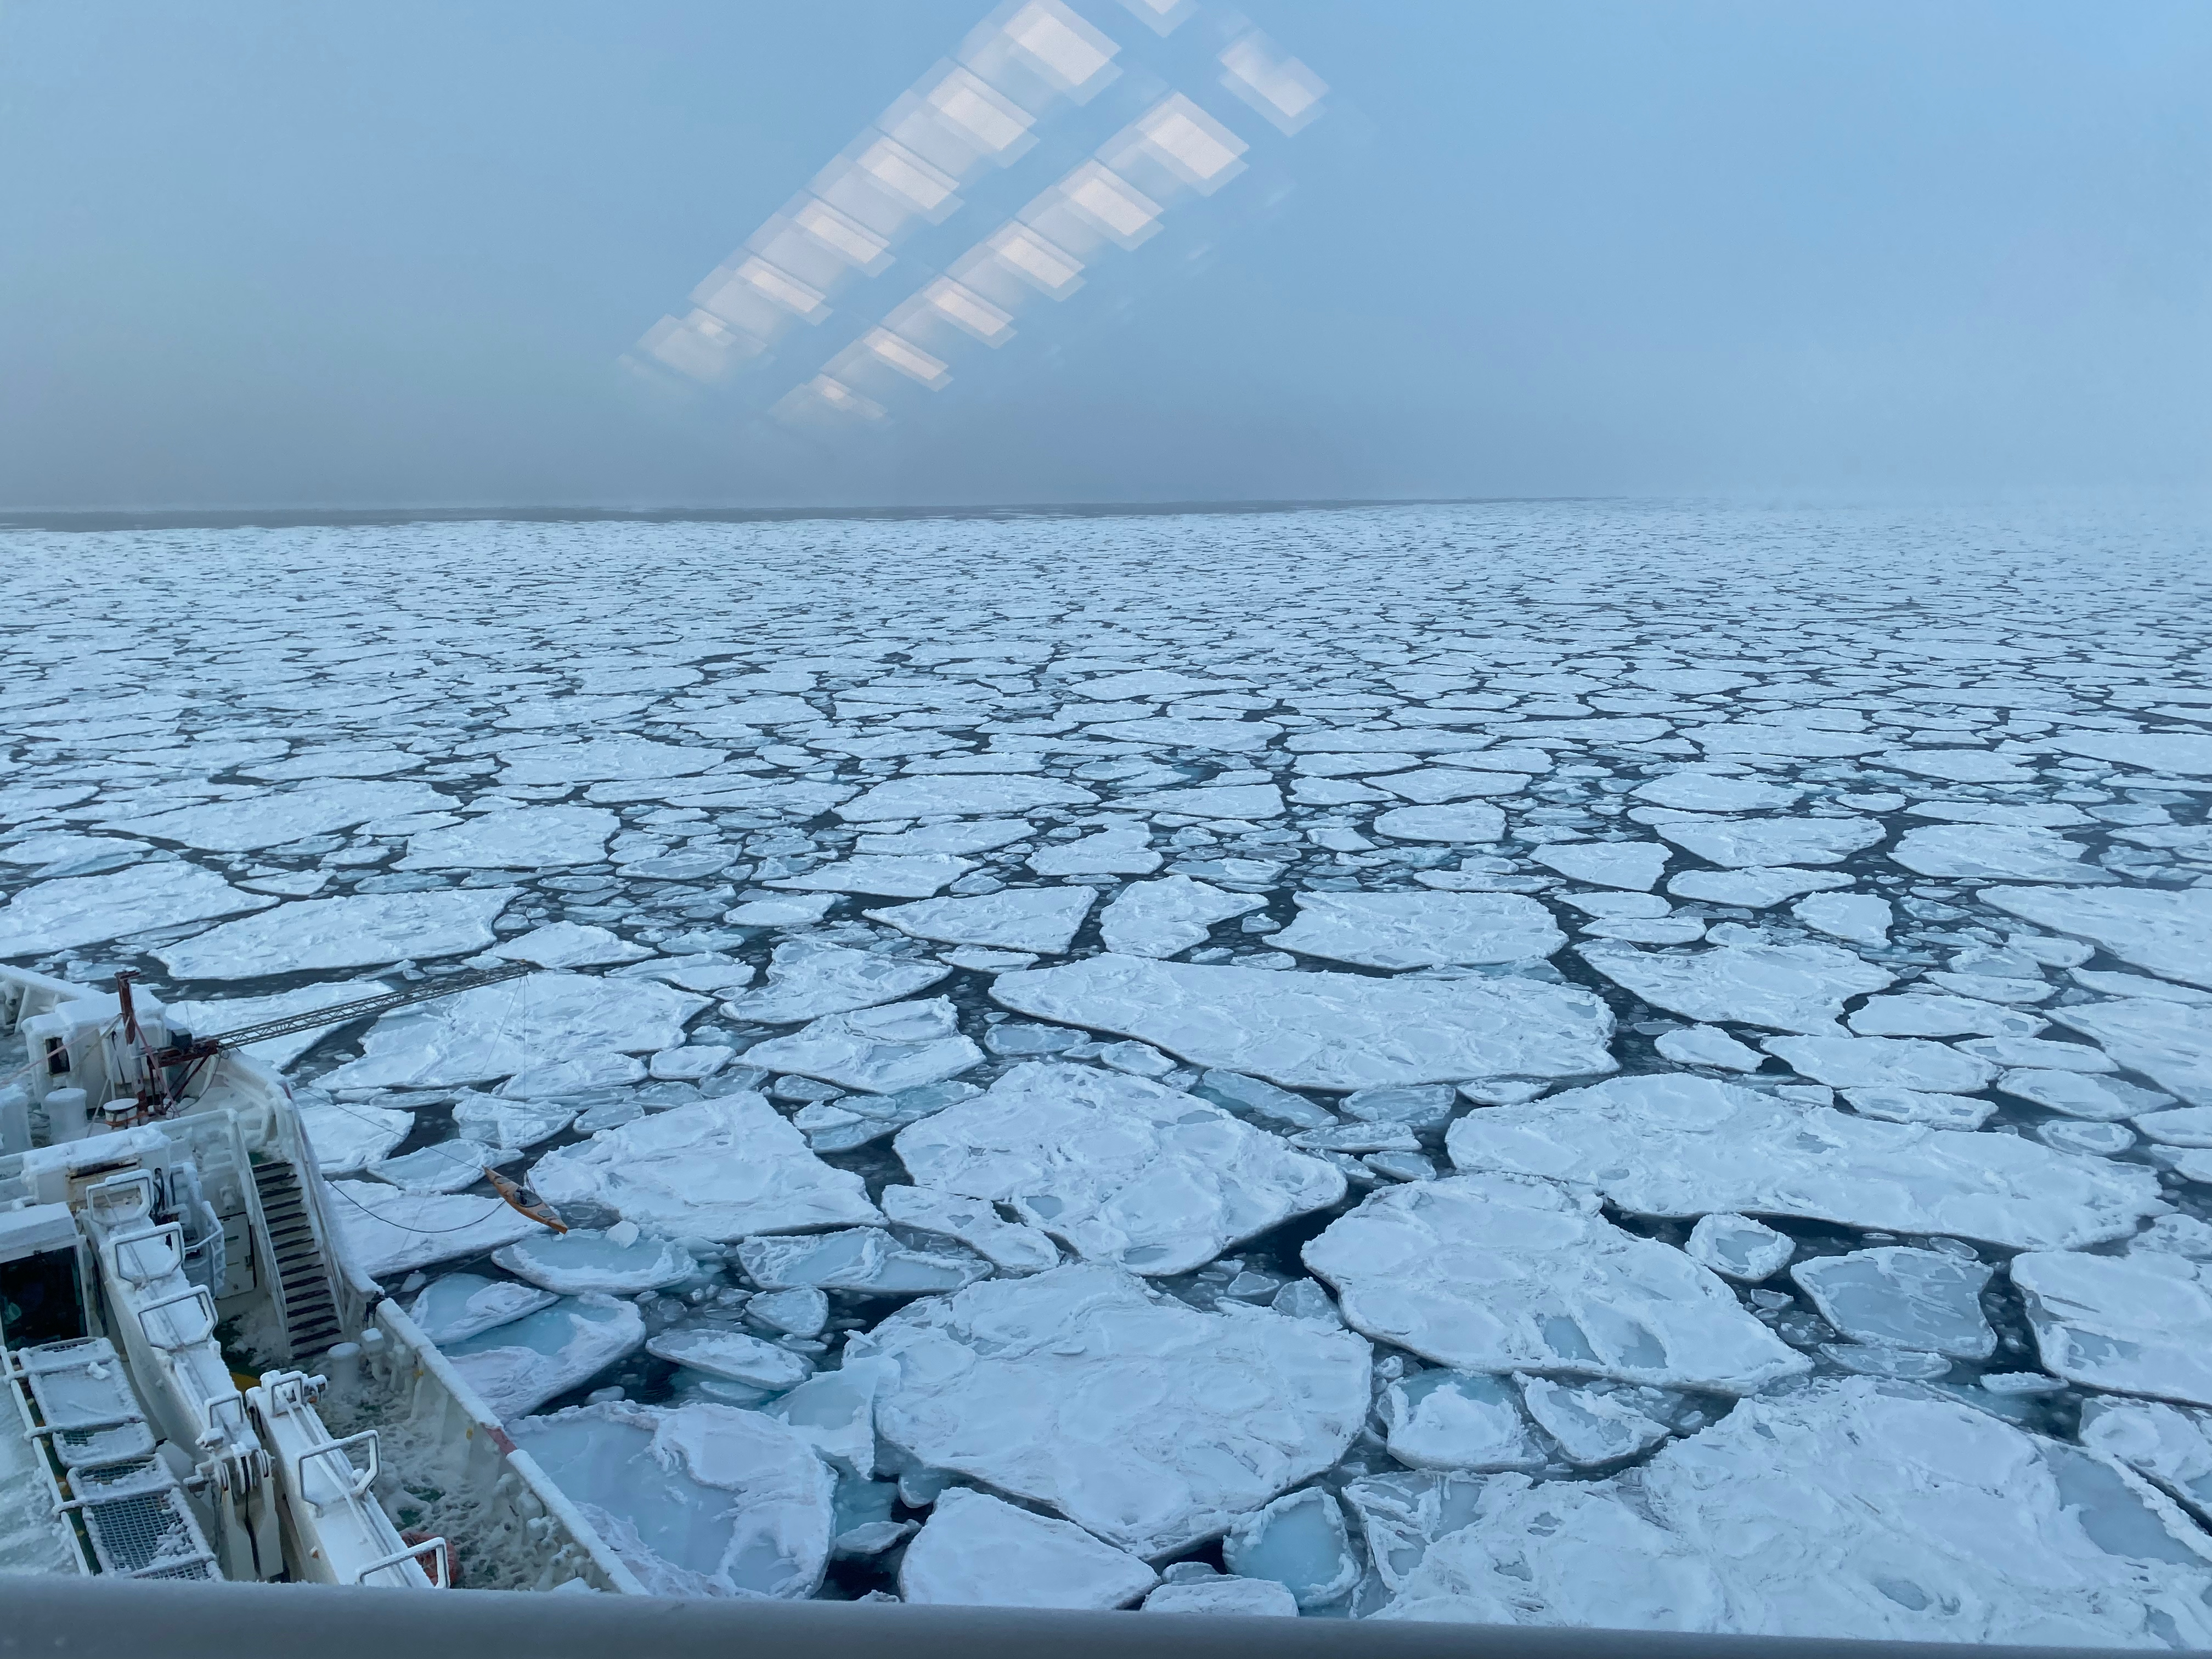
\includegraphics[width=0.5\textwidth]{figs/ch2/comp_pancake.jpeg}
    \caption{\textbf{Complex Ice Field.}}{Ice field likely created by a pancake floe sheet breaking apart. Captured during the SCALE Winter 2019 cruise aboard the \textit{S.A. Agulhas II}. Image credits: R.A. Verrinder.}
    \label{fig:comp_pancake}
\end{figure}
%----------------------------------------------------

These three stages of pancake ice formation are merely a conceptual model, and the exact processes by which Antarctic \ac{MIZ} young ice forms are still under investigation. The process of pancake ice formation is almost certainly not a linear one, with the stages likely overlapping and occurring simultaneously alongside other formation processes that we do not fully understand yet, as demonstrated by the widely varying pancake ice floe morphologies observed during the \ac{SCALE} Winter 2022 cruise (\cite{vichiSCALEWIN22CruiseReport2023}).

%====================================================
\section{Sea Ice-Environment Interactions}
\label{sec:ch2.section3}
%----------------------------------------------------

Sea ice interacts with its immediate environment in various ways, with the physical structure of the ice having the largest impact on the type and extent of interactions. Ice both reflects and transmits light, impacts environmental temperature, can dampen wave energy, interact with wind, and through freezing and melting, change the chemical composition of the surrounding seawater (\cite{roachPhysicsSeasonalSea2025}).

%----------------------------------------------------
\subsection{Wave-Ice Interactions}
\label{subsec:ch2.section3.subsec1}

In the Antarctic \ac{MIZ}, swell is the most common type of wave activity. Swell is initially generated by wind activity in the open ocean, where wind energy is transferred to the ocean surface, creating surface waves of lower amplitude and frequency than swell. These waves then constructively interfere with each other, leading to the formation of a wave field of higher amplitude and lower frequency than the original wind waves, which is what we refer to as swell (\cite{holthuijsenWavesOceanicCoastal2007}). Swell is then sustained by gravity, which is the primary force attempting to return the disturbance to equilibrium, and thus can propagate over long distances with little attenuation. The wave field in the Antarctic \ac{MIZ} consists mainly of wave energy with frequencies below 0.1 Hz (\cite{thomsonWavePropagationMarginal2022}). Under certain conditions and with sufficient energy, waves have the ability to propagate over 1000 km into pack ice (\cite{voermansFinelyresolvedAlongtrackWave2024}), propagation to this extent is rarely observed in the Arctic.

It is known that ocean surface waves are attenuated by sea ice as the waves travel through the \ac{MIZ} (\cite{williamsWaveIceInteractions2013}). The composition, structure and concentration of ice has an impact on the level of attenuation and thus, the distance the wave can travel through the ice field. If waves have sufficient energy it is also possible for the ice cover to be broken apart by wave action.

Wave activity also leads to interactions between individual ice floes, with collisions and rafting (when two floes overlap) occurring due to the motion induced by the waves (\cite{daiWaveRaftingEquilibrium2004}). The collisions between floes lead to the formation of distinct ridged edges on pancake ice floes, as seen in Figure \ref{fig:pancake_floes}. Rafting leads to the formation of composite floes, as discussed in Section \ref{subsec:ch2.section2.subsec3}.

%----------------------------------------------------
\subsection{Wind-Ice Interactions}
\label{subsec:ch2.section3.subsec2}

Wind not only drives the creation of wave activity, and the formation of pancake ice, but also directly interacts with the ice itself. Wind action on the ice surface leads to ice drift, with the ice being pushed in the direction of the wind. As \textcite{alberelloDriftPancakeIce2020} note, the drift of pancake ice is influenced by the surface roughness of the ice, with rougher surfaces leading to greater wind drag and thus faster drift speeds. The ridged edges of pancake ice floes, discussed in the Section above, are a significant contributor to the surface roughness of pancake ice.

The motion of pancake ice floes driven by wind action also leads to floe-floe interactions, such as collisions, as well as impacting the overall \ac{SIC} of the region. Wind activity can lead to an increase in wave activity, which in turn can lead to increased ice formation and growth, which in turn may cause a decrease in wave activity through floe-induced wave attenuation. This complex feedback loop between wind, waves and ice is still poorly understood.

%====================================================
\section{Antarctica and Remote Sensing}
\label{sec:ch2.section4}
%----------------------------------------------------

Satellite remote sensing has been the most common method for gathering data on the Antarctic region ever since satellite observation became widespread and the standard method for Earth observation and data collection. The methods for data collection have typically taken the form of \ac{SAR} imaging and Optical imaging (\cite{maslanikRemoteSensingAntarctica1990}). The use of lasers and \ac{LiDAR} in remote sensing is a recent development that has seen limited implementation in the past two decades (\cite{pettorelliSatelliteRemoteSensing2014}).

The first instance of optical imaging of the Antarctic took place in September 1964, when the Nimbus I satellite captured hundreds of greyscale images of the continent and surrounding ocean (\cite{meierNewEstimatesArctic2013}).
While the first use of \ac{SAR} to collect data over the Antarctic used the RADARSAT-1 satellite through the \ac{RAMP}, with the first phase of the project being completed in October 1997 (\cite{jezekRADARSAT1AntarcticMapping2002}).
Laser altimetry was first implemented aboard the \ac{ICESat}, through the \ac{GLAS}. \ac{ICESat} was a dedicated polar observation satellite, with the primary objective of monitoring the polar ice-sheets. The \ac{GLAS} produced elevation and atmospheric profiles and was launched in 2003, with data collection commencing in February of that year (\cite{schutzOverviewICESatMission2005}).
After the success of \ac{ICESat}, ICESat-2 was launched in September 2018, with the \ac{ATLAS} aboard the satellite. The \ac{ATLAS} sensor marked the first time a \ac{LiDAR} sensor was equipped to an observation satellite (\cite{palmICESat2AtmosphericChannel2021}).

Remote sensing has many advantages, it allows for long term, consistent data collection, large areas can be surveyed without the need for a physical presence in the region of interest, and it can be more cost-effective than in situ data collection. A brief comparison of the three main satellite-based remote sensing methods is given in Table \ref{tab:sense_comparison} (\cite{agrawalComparativeAssesmentRemote2019}).

%----------------------------------------------------
\begin{table}[H]
\centering
\caption{Satellite Remote Sensing Techniques Comparison.}{Optical, SAR and LiDAR remote sensing techniques are compared across various parameters, including sensor type, frequency range, spatial resolution, weather limitations, area coverage, data collected, data availability and technique maturity.}
\resizebox{\textwidth}{!}{%
\begin{tabular}{|l|l|l|l|}
\hline
\multicolumn{1}{|c|}{\textbf{Variable}} &
  \multicolumn{1}{c|}{\textbf{Optical}} &
  \multicolumn{1}{c|}{\textbf{\ac{SAR}}} &
  \multicolumn{1}{c|}{\textbf{\ac{LiDAR}}} \\ \hline
Sensor Type          & Passive            & Active                         & Active                 \\ \hline
Frequency Range      & 750 THz to 300 GHz & 300 GHz to 0.3 GHz             & 1 200 THz to 30 THz    \\ \hline
Spatial Resolution   & 30 m to 0.3 m      & 30 m to 0.3 m                  & 0.1 m to 0.02 m        \\ \hline
Weather Limitations  & Cannot penetrate cloud cover &  Can penetrate cloud cover &  Cannot penetrate heavy cloud cover \\ \hline
Area Coverage        & Large              & Large                          & Small                  \\ \hline
Data Collected       & Spectral Radiance  & Backscatter Amplitude \& Phase & Return Range Intensity \\ \hline
Data Availability    & Many datasets      & Many datasets                  & Few datasets           \\ \hline
Technique Maturity   & High               & Medium                         & Low                    \\ \hline
\end{tabular}%
}
\label{tab:sense_comparison}
\end{table}
%----------------------------------------------------

Due to their extreme locations, frequent adverse weather and polar night, \ac{SAR} has become the most common method for observing both the polar regions (\cite{comisoSatelliteRemoteSensing1991}). Despite the limited resources and harsh conditions, \ac{SAR} has greatly widened our knowledge of the Antarctic, allowing for tracking of sea ice coverage and extent, snow cover storms, biological activity, ice drift and iceberg calving (\cite{maslanikRemoteSensingAntarctica1990,dirscherlRemoteSensingIce2020,baumhoerRemoteSensingAntarctic2018}).

Currently, remote sensing falls short when attempting to identify the types of ice covering the ocean. \ac{SAR} imaging can estimate sea ice extent as well as sea ice concentration (regions where sea ice cover is present and regions that are open ocean). Information on the specific types of ice (grease, frazil, nilas, pancake, etc.) is virtually impossible to extract from \ac{SAR} data alone (\cite{zakhvatkinaSatelliteSARDatabased2019}).

%----------------------------------------------------
\subsection{LiDAR}
\label{subsec:ch2.section4.subsec1}

\ac{LiDAR} is an active remote sensing technique that uses laser pulses to build a three-dimensional point cloud. A point cloud is a set of discrete points in a coordinate space that represent the geometry of a target. A point cloud is created by the sensor sending a laser pulse toward the target, recording the returned signal, and using the time of flight (or phase shift) and the direction in which the pulse was propagated to determine target range and position (\cite{kukkoMobileLaserScanning2013}). By repeating this process rapidly across different directions, a complete point cloud of the target scene is created.

The development of modern \ac{LiDAR} began with the invention of lasers, which initially led to the development of simple laser rangefinders in the 1960s. These early rangefinders were capable of measuring the distance to a single target less than 5 km away to an accuracy of 2 to 3 m and were primarily used for military applications (\cite{molebnyLaserRadarHistorical2016}). Beginning in the 1970s and through to the 1980s, airborne laser rangefinders were first used for Earth observation, with applications ranging from sea ice surface roughness, bathymetric and topographical measurements (\cite{nelsonHowDidWe2013}).

Once again, military applications led the development of \ac{LiDAR} technology, with the first true \ac{LiDAR} systems capable of producing full three-dimensional point clouds being developed in the 1980s. These systems were initially heavy, large and required significant power to operate, leading to their deployment being limited to large, vehicle-mounted platforms (\cite{molebnyLaserRadarHistorical2016}).  

%----------------------------------------------------
\begin{figure}[H]
\centering
\begin{minipage}{.5\textwidth}
    \centering
    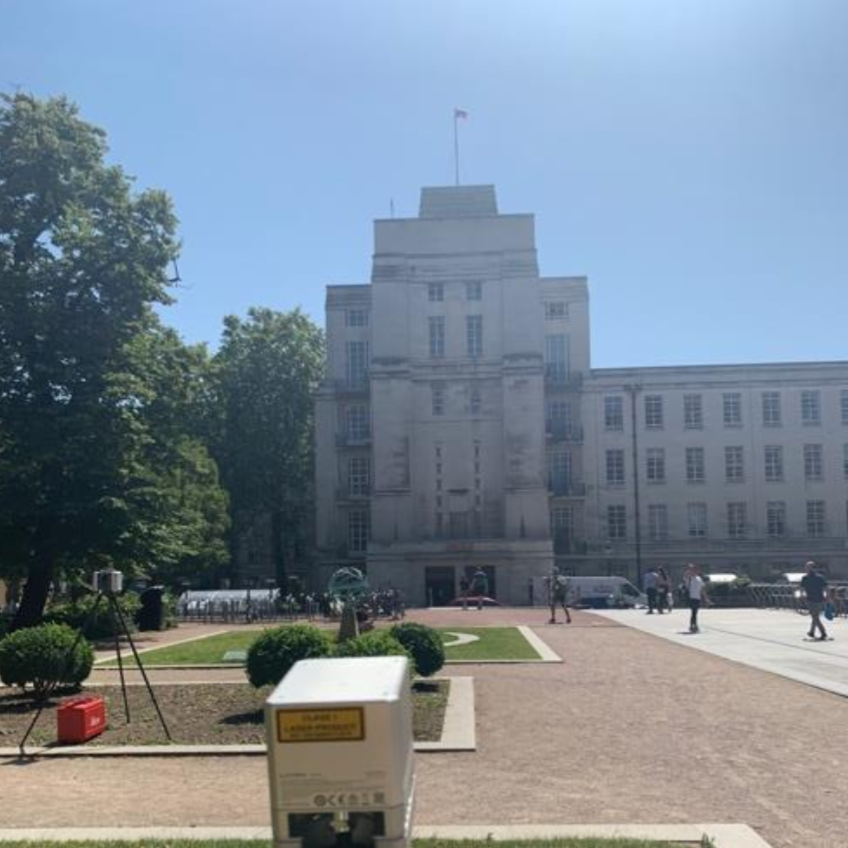
\includegraphics[width=\linewidth]{figs/ch2/image.png}
  \end{minipage}%
  \begin{minipage}{.5\textwidth}
    \centering
    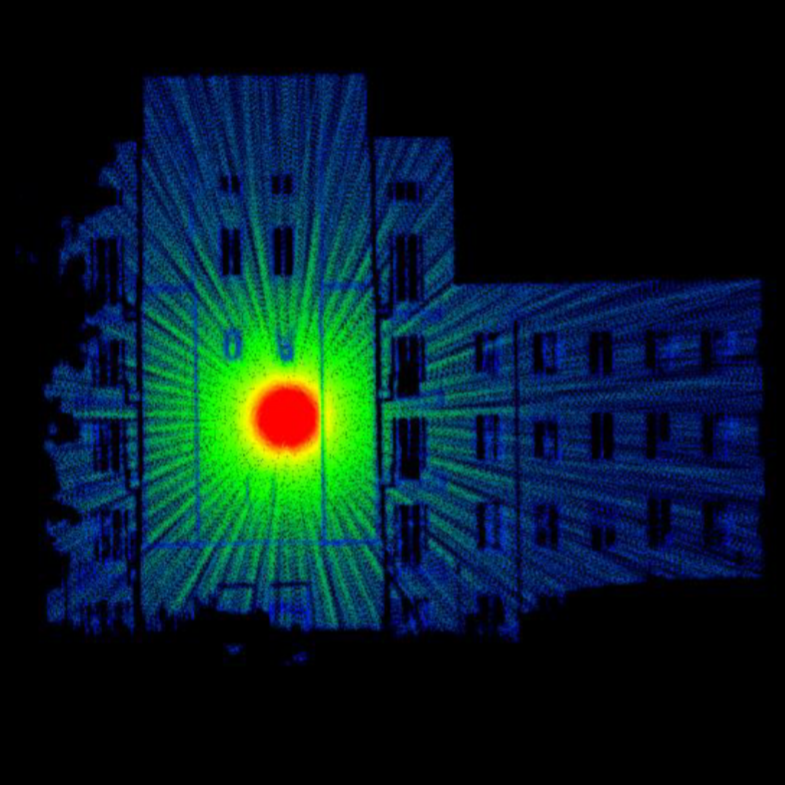
\includegraphics[width=\linewidth]{figs/ch2/pointcloud.png}
  \end{minipage}
  \caption{\textbf{Image and Point Cloud Comparison.}}{Left: Image of a target scene. Right: Point cloud of the same scene (colours represent point density) created by Livox MID-40, a similar sensor to the Livox Avia used in this investigation. Images are capable of capturing details such as colour and texture, while point clouds capture the geometry of the scene. Taken from \textcite{ortizarteagaInitialInvestigationLowCost2019}.}
  \label{fig:cam_vs_lidar}
\end{figure}
%----------------------------------------------------

Commercial \ac{LiDAR} systems first became available in the early 2000s, with advancements laser, processing and power delivery systems leading to smaller, lighter and more power efficient sensors at lower costs. This has resulted in \ac{LiDAR} becoming more accessible to a wider range of applications and has opened up new possibilities and potential applications (\cite{wangEvolutionLiDARIts2020}). \ac{LiDAR} has seen limited deployment in Antarctica, with \textcite{sandruShipborneSeaiceField2021} being potentially the first instance of making use of \ac{LiDAR} for the mapping of sea ice from aboard the \textit{S.A. Agulhas II}. They were able to successfully create a point cloud reconstruction of the sea ice field surrounding the vessel to assist in the potential autonomous navigation of vessels through ice-covered waters. This investigation demonstrated that ship-based \ac{LiDAR} is capable of producing point cloud reconstructions of sea ice fields, and thus has the potential to be used as an observational tool in Antarctica. With further development and investigation, it may be possible to determine parameters such as individual pancake ice floe size and distribution, as well as wave-in-ice parameters such as wave amplitude and period.

%====================================================
\section{Summary}
\label{sec:ch2.section5}
%----------------------------------------------------

Antarctica and the Southern Ocean are vital components of the Earth's environmental system, and while research and interest in the regions have increased significantly in recent years, many aspects of their behaviour and dynamics are still poorly understood. Sea ice dynamics, particularly those of the \ac{MIZ} during the winter months, are one such area where large gaps in our understanding persist. 

These gaps in our understanding of the \ac{MIZ} are a clear indication that further investigation into the dynamics of the region is necessary. Historically, satellite remote sensing has been the most common method for gathering data on the Antarctic region, with \ac{SAR} and optical imaging being the most widely used techniques. The use of \ac{LiDAR} in remote sensing is a recent development that has seen limited implementation in the past two decades, its use as an observational tool in Antarctica has the potential to greatly enhance our understanding of the region, particularly in relation to sea ice dynamics and wave-ice interactions.

By improving our understanding of floe-level parameters and dynamics, particularly during their formation and growth stages, progress can be made towards reducing the uncertainties and biases present in current data and models of the Antarctic.

%****************************************************
% END
%****************************************************